\documentclass{IEEEtran}

\usepackage{graphicx}
\usepackage{amsthm}
\usepackage{amssymb}
\usepackage{amsmath}
\usepackage{algorithm}
\usepackage{algorithmicx}
\usepackage{algpseudocode}
\usepackage{booktabs}
\usepackage{color}

\newcommand{\comment}[1]{}

%\renewcommand{\baselinestretch}{0.95}
%\setlength{\textfloatsep}{0.1cm}
%\setlength{\abovecaptionskip}{0.1cm}

\begin{document}

\title{Preserving Differential Privacy on Ranked Similarity Search over Encrypted Cloud Data}
\author{
Shiyu Ji}
\maketitle

\newtheorem{definition}{Definition}
\theoremstyle{definition}
\newtheorem{theorem}{Theorem}
\theoremstyle{plain}
\newtheorem{lemma}{Lemma}
\theoremstyle{plain}
\newtheorem{corollary}{Corollary}
\theoremstyle{plain}

\section{Problem Formulation}
\subsection{The System and Threat Model}

\begin{figure}
\centering
\includegraphics[width=0.45\textwidth]{system_model.eps}
\caption{The architecture of ranked similarity search over encrypted cloud data.}
\label{fig:system_model}
\end{figure}

As in Fig. \ref{fig:system_model}, we consider a cloud data hosting service which consists of three entities: the data owner, the data users and the semi-trusted cloud data server. The data owner has a collection of documents that need to be outsourced to the semi-trusted cloud server. The outsourced documents must be encrypted since the data owner does not want to reveal the documents to the semi-trusted server. The encryption scheme will be given later. On the other hand, the data users want to search over the encrypted documents. To enable this, the data owner prepares a search index of the outsourced documents, and then uploads the encrypted index to the server. On a similarity search request, an authorized data user firstly gets the corresponding trapdoors and keys from the data owner, and uses the keys to encrypt the query, and then sends the encrypted search query to the cloud server. Upon receiving the search query, the server should securely search on the index and return the top $k$ most similar documents in the encrypted form to the user.

We assume the cloud server is \emph{semi-trusted}, or \emph{honest-but-curious}, i.e., the server will honestly do as described above, but it also wants to know any information of the outsourced documents and the submitted search queries. We consider the \emph{Ciphertext-Only Attack}, in which the server only has the submitted encrypted documents and queries, but it initially has no knowledge about their plaintext. We will also consider another stronger attack, in which we assume the server has some knowledge about the outsourced content, e.g., the frequency distribution. Thus some statistical attacks may be launched.

\subsection{Our Goals}
We want to design an efficient and secure ranked search scheme over encrypted cloud data that satisfy the requirements above, and we also want it to keep privacy to some extent.

\textbf{Efficiency}. The algorithms should be efficient, e.g., 1) encryption over the documents, index and queries, 2) search over the encrypted index, etc.

\textbf{Dynamic updating support}. The data owner should be able to update the documents and index efficiently at any time.

\textbf{Confidentiality}. The content of the documents, the entries in the index and the submitted queries should not be revealed to the cloud server.

\textbf{Privacy preserving}. We want to prevent the cloud server from learning anything about the outsourced documents, index or queries submitted by users. We will investigate the cases as follows:
\begin{itemize}
\item \textbf{Query unlinkability}. The server should be difficult to tell whether two encrypted queries are from the same search request (e.g., the same keywords or terms) if these two queries are generated by similar search requests. Note the server can easily tell apart the queries from very different requests, since the returned top $k$ documents could be very different.
\item \textbf{Keyword privacy}. The server should not know any information about the keywords or terms in the search request.
\end{itemize}

\subsection{Notations and Preliminaries}
\begin{itemize}
\item $\mathbf{F}$ \---- The collection of the documents to be outsourced: $\mathbf{F} = \{f_1, f_2, \cdots, f_n\}$ where $f_i$ denotes the $i$-th document.
\item $\mathbf{C}$ \---- The collection of the encrypted documents in $\mathbf{F}$: $\mathbf{C} = \{c_1, c_2, \cdots, c_n\}$ where each $c_i$ is the encrypted form of $f_i$.
\item $I$ \---- The index built for $\mathbf{C}$: $I = \{I_1, I_2, \cdots, I_n\}$. Denote by $I_i$ the entry of $c_i$. Each $I_i$ is a vector determined by the keywords and terms in $f_i$.
\item $\mathbf{W}$ \---- The set of the keywords and terms: $\mathbf{W} = \{W_1, W_2, \cdots, W_m\}$.
\item $r$ \---- The search request $r$, which contains the keywords and terms that are interesting to the user.
\item $q$ \---- The query vector determined by the keywords and terms in the search request $r$.
\item $\hat{F}$ \---- The top $k$ documents: $\hat{F} = \{\hat{f}_1, \hat{f}_2, \cdots, \hat{f}_k\}$ with the highest similarities to the query $q$.
\item $v[i]$ \---- The $i$-th component of the vector $v$.
\end{itemize}

\emph{Cosine similarity} is a popular measure to evaluate the similarity between two vectors in information retrieval \cite{ATY13,TAJY14}. Given a set of vectors $v_i = (v_{i,1}, v_{i,2}, \cdots, v_{i,m})^T$ where each vector is normalized to a unit length, and has at most $m$ features (if $v_i$ does not have feature $k$, we can set $v_{i,k}$ to be zero), the cosine similarity between vectors is defined as follows:
$$Sim(v_i,v_j) = \sum_{k=1}^m v_{i,k}\cdot v_{j,k}.$$
Note that the cosine similarity of two vectors equals to their dot product. We say two vectors are similar if their cosine similarity exceeds some threshold $\tau$. For a ranked search over the documents $\mathbf{F}$, given the query vector $q$, we want the cloud server to return the top $k$ documents $\{\hat{f}_i\}$ with the highest cosine similarities $Sim(\hat{f}_i, q)$.

\emph{Differential privacy} \cite{Dwork08,DR14} is a popular measure for privacy preserving analysis. 
\begin{definition}
We say a randomized algorithm $A$ achieves $\epsilon$-differential privacy if for all data sets $D_i$ and $D_j$ differing on at most one element, and for all subsets $S$ in the range of $A$ (viewed as a function),
\begin{equation}
\label{eqn:dp}
\Pr[A(D_i) \in S] \leq \exp(\epsilon)\cdot \Pr[A(D_j)\in S],
\end{equation}
where the probability is taken over all the random choices of $A$.
\end{definition}
We will use differential privacy to study query unlinkability. Let each data set be a collection of $n$ independently sampled query pairs: 
$$D_i = \{(q_{i,1}^1, q_{i,2}^1), (q_{i,1}^2, q_{i,2}^2), \cdots, (q_{i,1}^n, q_{i,2}^n)\}.$$
For each data set, the two queries in each pair are either from the same search request, or from two requests $r_1$, $r_2$ with similarity distance $d$, i.e., for any normalized vector $v$, $|Sim(v,r_1) - Sim(v,r_2)| \leq d$. This is the only differing element among $D_i$'s. The attacker gives an algorithm $A$ deciding whether the queries in $D_i$ are from the same request or not. Thus $A$ only outputs a bit: $Range(A) = \{0,1\}$. If for any efficient algorithm $A$, Eq. (\ref{eqn:dp}) holds, then we say our search scheme preserves $\epsilon$-differential privacy under the parameters $(n, d)$.

Based on the above, the secure ranked similarity search scheme can be summarized as follows:
\begin{itemize}
\item \textbf{Setup}($1^\lambda$): the data owner takes a security parameter $\lambda$ as input and generates a private key $sk$ that will be used to encrypt the outsourced documents.
\item \textbf{BuildIndex}($\mathbf{F}$, $sk$): using the key $sk$, the data owner builds an encrypted index $I$ given the documents $\mathbf{F}$. Each entry $I_i$ is an encrypted vector determined by the keywords and terms contained in the document $f_i$.
\item \textbf{Query}($\mathbf{W}$, $r$): the authorized user computes the query vector $q$ based on the keywords and terms in the search request $r$, and sends the vector $q$ to the cloud server. We want the queries $q$'s to achieve differential privacy to some extent.
\item \textbf{Search}($q$, $\mathbf{C}$): the cloud server searches over the encrypted documents $\mathbf{C}$ and determines the top $k$ documents $\hat{F}$ that are the most similar to the query vector $q$. We want the server can figure out the most similar $k$ documents as accurate as possible given the encrypted $q$ and index entries $I_i$.
\end{itemize}

\section{Our Proposed Schemes}
In this section we firstly recall the secure dot product encryption \cite{Cao14} (which was adapted from \cite{Wong09}). Then we propose our scheme for ranked similarity search.

\subsection{Secure Dot Product Encryption}
In Cao et al's scheme \cite{Cao14}, the cloud server can approximately compute the dot product between an index entry $I_i$ and the query vector $q$. The private key $sk$ consists of a $(m+2)$-bit string $S$ and two $(m+2)\times (m+2)$ invertible matrices $M_1$ and $M_2$, where $m$ is the number of features in each vector. To encrypt, we add two more dimensions to both $I_i$ and $q$ (we denote the extended vectors as $D_i$ and $Q$ respectively): 1) for all $D_i$, the $D_i[m+1]$ is set to a random number $\varepsilon_i$, and $D_i[m+2]$ is set to 1; 2) the $Q[m+1]$ is set to 1, and then the first $(m+1)$ components are scaled by a non-zero random number $r$, and finally $Q[m+2]$ is set to another independent random number $t$. Then $D_i$ is split into two random vectors $D_i'$ and $D_i''$, and $Q$ is also randomly split into $Q'$ and $Q''$. The string $S$ is a splitting indicator: if the $k$-th bit of $S$ is 0, then the $D_i'[k]$ and $D_i''[k]$ are the same as the $D_i[k]$, while the sum of $Q'[k]$ and $Q''[k]$ should be the $Q[k]$; if the $k$-th bit of $S$ is 1, then the process is similar except that the positions of $D_i$ and $Q$ are exchanged. The split index entry is encrypted as $(M_1D_i', M_2D_i'')$, and the split query vector is encrypted as $(M_1^{-1}Q', M_2^{-1}Q'')$. Upon an encrypted query $Q$, the cloud server computes the approximate dot product given encrypted $D_i$ as follows:
\begin{equation*}
\begin{aligned}
&(M_1D_i', M_2D_i'')\cdot(M_1^{-1}Q', M_2^{-1}Q'') \\
=&D_i'\cdot Q' + D_i''\cdot Q''\\
=&\sum_{S[k]=1}D_i[k](Q'[k] + Q''[k]) + \sum_{S[j]=0} (D_i'[j]+ D_i''[j])Q[j]\\
=&\sum_{S[k]=1}D_i[k]Q[k] + \sum_{S[j]=0} D_i[j]Q[j]\\
=&D_i \cdot Q = (I_i,\varepsilon_i,1)\cdot (rq,r,t)\\
=&r(I_i\cdot q+\varepsilon_i)+t.
\end{aligned}
\end{equation*}
Clearly if the bounds of the random $\varepsilon_i$ and $t$ are small enough, the result is approximately proportional to $Sim(I_i, q)$. In \cite{Cao14} $\varepsilon_i$ is considered when computing similarity between $I_i$ and any query $q$. However in this paper we use cosine similarity, and thus we can set each $\varepsilon_i$ to be zero or some very small value. Then the result is close to $rI_i\cdot q+t$. 
Note that only $r$ and $t$ are not enough to preserve privacy, since they can be easily reverse-engineered: suppose the cloud server collects extensive $rI_i\cdot q+t$ values by fixing $q$, then
\begin{itemize}
\item often there exists an index entry $I_k$ that is very distinct from $q$. $I_k$ gives an almost zero similarity and thus $t$ is completely compromised by finding the lowest value of $rI_i\cdot q+t$. And
\item the highest value of them can probably be used to estimate $r$ since the maximum similarity $I_i\cdot q$ can usually be learned from historic search experience. 
\end{itemize}
Thus we need to introduce more randomness to better preserve privacy, e.g, the similarity, the query unlinkability, etc.

\subsection{Improved Scheme}
We observe that the above scheme is not secure since all the ``safeguard'' random numbers are associated to the query side, but none of them is chosen by the index side. Hence the basic idea of our improved scheme is to introduce a random number during the encryption of index entries.


\section{Security Analysis}

\bibliographystyle{./IEEEtran}
\bibliography{./sim_privacy}
\end{document}
